\section{Mathematical model}
\label{sec:math}

\subsection{Motion laws}
\label{sec:motion}

The complete set of equations is continuous, non-linear and couples the two modes
of motion. After a discretization and linearization process about the operating
point, which is the equilibrium configuration
($x = y = \theta_x = \theta_y = 0$), the equations of motion for the ball,
along the $x$ and $z$ axis, are the following:

\begin{align*}
\ddot{x}[k] &= \frac{5}{7}\ g\ sin (\theta_x[k]) - \left ( r_b + \frac{5}{7}\ h \right ) \dot{\omega}_x[k];\\
%\frac{7}{5} \ddot{y} + \left ( \frac{7}{5} r_b + h \right ) \dot{\omega}_y &= g sin (\theta_y)
m\ddot{z}[k] &= N - mg\ cos(\theta_x[k]) = 0;\\
%\dot{x}[k] &= \frac{ x[k] - x[k-1] } {\Delta t}\\
\dot{x}[k] &= \ddot{x}[k] \Delta t + \dot{x}[k-1];\\
x[k] &= \dot{x}[k] \Delta t + x[k-1];\\
\omega[k] &= \frac{ \theta[k] - \theta[k-1] } {\Delta t};\\
\dot{\omega}[k] &= \frac{ \omega[k] - \omega[k-1] } {\Delta t}.
\label{eq:kinematic}
\end{align*}

Where $\Delta t$ is the updating period (the time elapsed since the previous
check event until the actual). The first two equations are computed
according to the Newton's laws and the last four by the classical kinematic
formulas, assuming a motion uniformly accelerated during each $\Delta t$.

The final kinematic formula to model the ball motion is shown in
Equation~\ref{eq:final_kinematic}.
\begin{equation}
\begin{aligned}
	x[k] &= \ddot{x}[k] \Delta t^2 + \dot{x}[k-1] \Delta t + x[k-1] =\\
		 &= \left[ \frac{5}{7}g \sin(\theta_x[k]) - \left( r_b + \frac{5}{7} h \right) \dot{\omega}_x[k] \right] \Delta t^2 +
			\dot{x}[k-1] \Delta t + x[k-1].
\end{aligned}
\label{eq:final_kinematic}
\end{equation}

\subsection{Angles}
\label{sec:angles}

The relation between $\alpha$ and $\theta$ is given by the closed chain geometry
(considering negligible the elastic coefficient of the plate structure).

\begin{equation}
\left\{
\begin{aligned}
	\hat{x}: & \quad l\ cos(\theta) + h\ sin(\theta) = D + r\ cos(\alpha) + b\ sin(\gamma)\\
	\hat{y}: & \quad H + l\ sin(\theta) = r\ sin (\alpha) + b\ cos(\gamma) + h\ cos(\theta)
\end{aligned}
\right.
\label{eq:basic_model}
\end{equation}

The angle $\gamma$ can be removed and, exploiting the trigonometric axiom
$sin(\beta)^2+cos(\beta)^2=1$, the problem can be rewritten as:

\begin{equation}
[H + l\ sin(\theta) - r\ sin (\alpha) - h\ cos(\theta)]^2 +
[l\ cos(\theta) + h\ sin(\theta) - D - r\ cos(\alpha)]^2 = b^2.
\label{eq:simple_model}
\end{equation}

The relation $\theta = f(\alpha)$ which binds the servomotor angle and the plate
inclination can be better formulated solving Equation~\ref{eq:simple_model}.

\begin{equation}
\begin{aligned}
1: \quad & \{[H + l\ sin(\theta)] - [r\ sin (\alpha) + h\ cos(\theta)]\}^2 + \{[l\ cos(\theta) + h\ sin(\theta)] - [D + r\ cos(\alpha)]\}^2 = b^2;\\
2: \quad & [H + l\ sin(\theta)]^2 + [r\ sin (\alpha) + h\ cos(\theta)]^2 - 2 [H + l\ sin(\theta)][r\ sin (\alpha) + h\ cos(\theta)] +\\
   & + [l\ cos(\theta) + h\ sin(\theta)]^2 + [D + r\ cos(\alpha)]^2 - 2 [l\ cos(\theta) + h\ sin(\theta)] [D + r\ cos(\alpha)]= b^2;\\
3: \quad & H^2 + l^2 sin(\theta)^2 + 2 H l sin(\theta) + r^2 sin (\alpha)^2 + h^2 cos(\theta)^2 + 2 r h sin (\alpha) cos(\theta) +\\
   & - 2 H r sin (\alpha) -2 l r sin(\theta) sin(\alpha) -2 H h cos(\theta) -2 l h sin(\theta) cos(\theta) +\\
   & + l^2 cos(\theta)^2 + h^2 sin(\theta)^2 + 2 l h cos(\theta) sin(\theta) + D^2 + r^2 cos(\alpha)^2 + 2 D r cos(\alpha) +\\
   & - 2 l D cos(\theta) - 2 l r cos(\theta) cos(\alpha) - 2 h D sin(\theta) -2 h r sin(\theta) cos(\alpha)= b^2;\\
4: \quad & b^2 = H^2 + l^2 + r^2  + h^2 + D^2 + 2 D r cos(\alpha) - 2 H r sin(\alpha) +\\
   & + 2 cos(\theta) [ h r sin(\alpha) - H h - l D - l r cos(\alpha) ] + 2 sin (\theta) [ H l - l r sin(\alpha) - h D - r h cos(\alpha)].
\end{aligned}
\label{eq:f_alpha}
\end{equation}

In order to make the model easier, it is linearized considering small swings of
$\theta$ which means that $sin(\theta)=\theta$ and $cos(\theta)=1$.
From this perspective, the result of Equation~\ref{eq:f_alpha} can be rewritten
as reported in Equation~\ref{eq:f_alpha_small_swings}.

\begin{equation}
\begin{aligned}
& b^2 = H^2 + l^2 + r^2  + h^2 + D^2 + 2 D r cos(\alpha) - 2 H r sin(\alpha) +\\
& + 2 [ h r sin(\alpha) - H h - l D - l r cos(\alpha) ] + 2 \theta [ H l - l r sin(\alpha) - h D - r h cos(\alpha)].
\end{aligned}
\label{eq:f_alpha_small_swings}
\end{equation}

Expressing the formula in function of $\theta$ will lead to
Equation~\ref{eq:theta}.

\begin{equation}
\theta = \frac{H^2 + l^2 + r^2  + h^2 + D^2 + 2 D r cos(\alpha) - 2 H r sin(\alpha) - b^2 + 2 [ h r sin(\alpha) - H h -
l D - l r cos(\alpha) ]}{2 [ l r sin(\alpha) + h D + r h cos(\alpha) - H l]}.
\label{eq:theta}
\end{equation}

Although the plate is in a rest position ($\theta=0^{\circ}$) when the 
servomotor is ordered to hold $0^{\circ}$, the actual $\alpha$ is not
$0^{\circ}$ according to how the ball and plate models have been designed.

$\alpha_{x0}$ and $\alpha_{y0}$ are computed, imposing $\theta=0^{\circ}$ as
shown in Equation~\ref{eq:equilibrium}.
\begin{equation}
\left\{
\begin{aligned}
	\hat{x}: & \quad [H - r\ sin (\alpha_{x0}) - h]^2 + [l - D - r\ cos(\alpha_{x0})]^2 = b^2\\
	\hat{y}: & \quad [H - r\ sin (\alpha_{y0}) - h]^2 + [l - D - r\ cos(\alpha_{y0})]^2 = b^2
\end{aligned}
\right.
\label{eq:equilibrium}
\end{equation}

For the sake of simplicity, the calculus refers only to $x$ axes and it is
reporter in Equation~\ref{eq:equilibrium_1}
\begin{equation}
\left\{
\begin{aligned}
&	A \sin(\alpha) + B \cos(\alpha) + C = 0\\
&	A = 2rh-2Hr\\
&	B = 2Dr-2lr\\
&	C = H^2+r^2+h^2+l^2+D^2-b^2-2Hh-2lD
\end{aligned}
\right.
\label{eq:equilibrium_1}
\end{equation}

In order to solve the trigonometric equation imposing $t=\tan(\frac{x}{2})$
lets us transform the problem into a second order equation, as shown in
Equation~\ref{eq:equilibrium_2}.

\begin{equation}
\left\{
\begin{aligned}
&	t=\tan(\frac{x}{2})\\
&	(C-B)\ t^2 + 2A\ t + B + C = 0
\end{aligned}
\right.
\label{eq:equilibrium_2}
\end{equation}

According to the model parameters defined in Table~\ref{tab:measurements},
the equilibrium angles are $\alpha_{x0}\simeq-38.814^{\circ}$ ($-0.68$ rad) and
$\alpha_{y0}\simeq-30^{\circ}$ ($-0.52$ rad).

For this reason, $\alpha$ needs to be consider as the sum between the rest angle
and the desired angle: $\alpha = \alpha_0 + \alpha'$.

Considering small swings for $alpha$ and the addition formulas\footnotemark,
 trigonometric operations in Equation~\ref{eq:theta} are rewritten as:
\begin{equation}
\begin{aligned}
sin(\alpha) =& \alpha' cos(\alpha_0) + sin(\alpha_0);\\
cos(\alpha) =& cos(\alpha_0) - \alpha' sin(\alpha_0).
\end{aligned}
\label{eq:new_theta}
\end{equation}

\footnotetext[1]{
Addition formulas:
\begin{itemize}
    \item $\sin(\alpha + \beta) = \sin(\alpha) \cos(\beta) + \cos(\alpha) \sin(\beta)$;
    \item $\cos(\alpha + \beta) = \cos(\alpha)\cos(\beta) - \sin(\alpha)\sin(\beta)$.
\end{itemize}
}

The plot of the function $\theta = f(\alpha)$ is depicted in
Figure~\ref{fig:f_alpha} (with $\alpha \in [0, \pi]$), where in $\alpha=2.25$ a
vertical asymptote occurs.

\begin{figure}[htb]
  \centering

  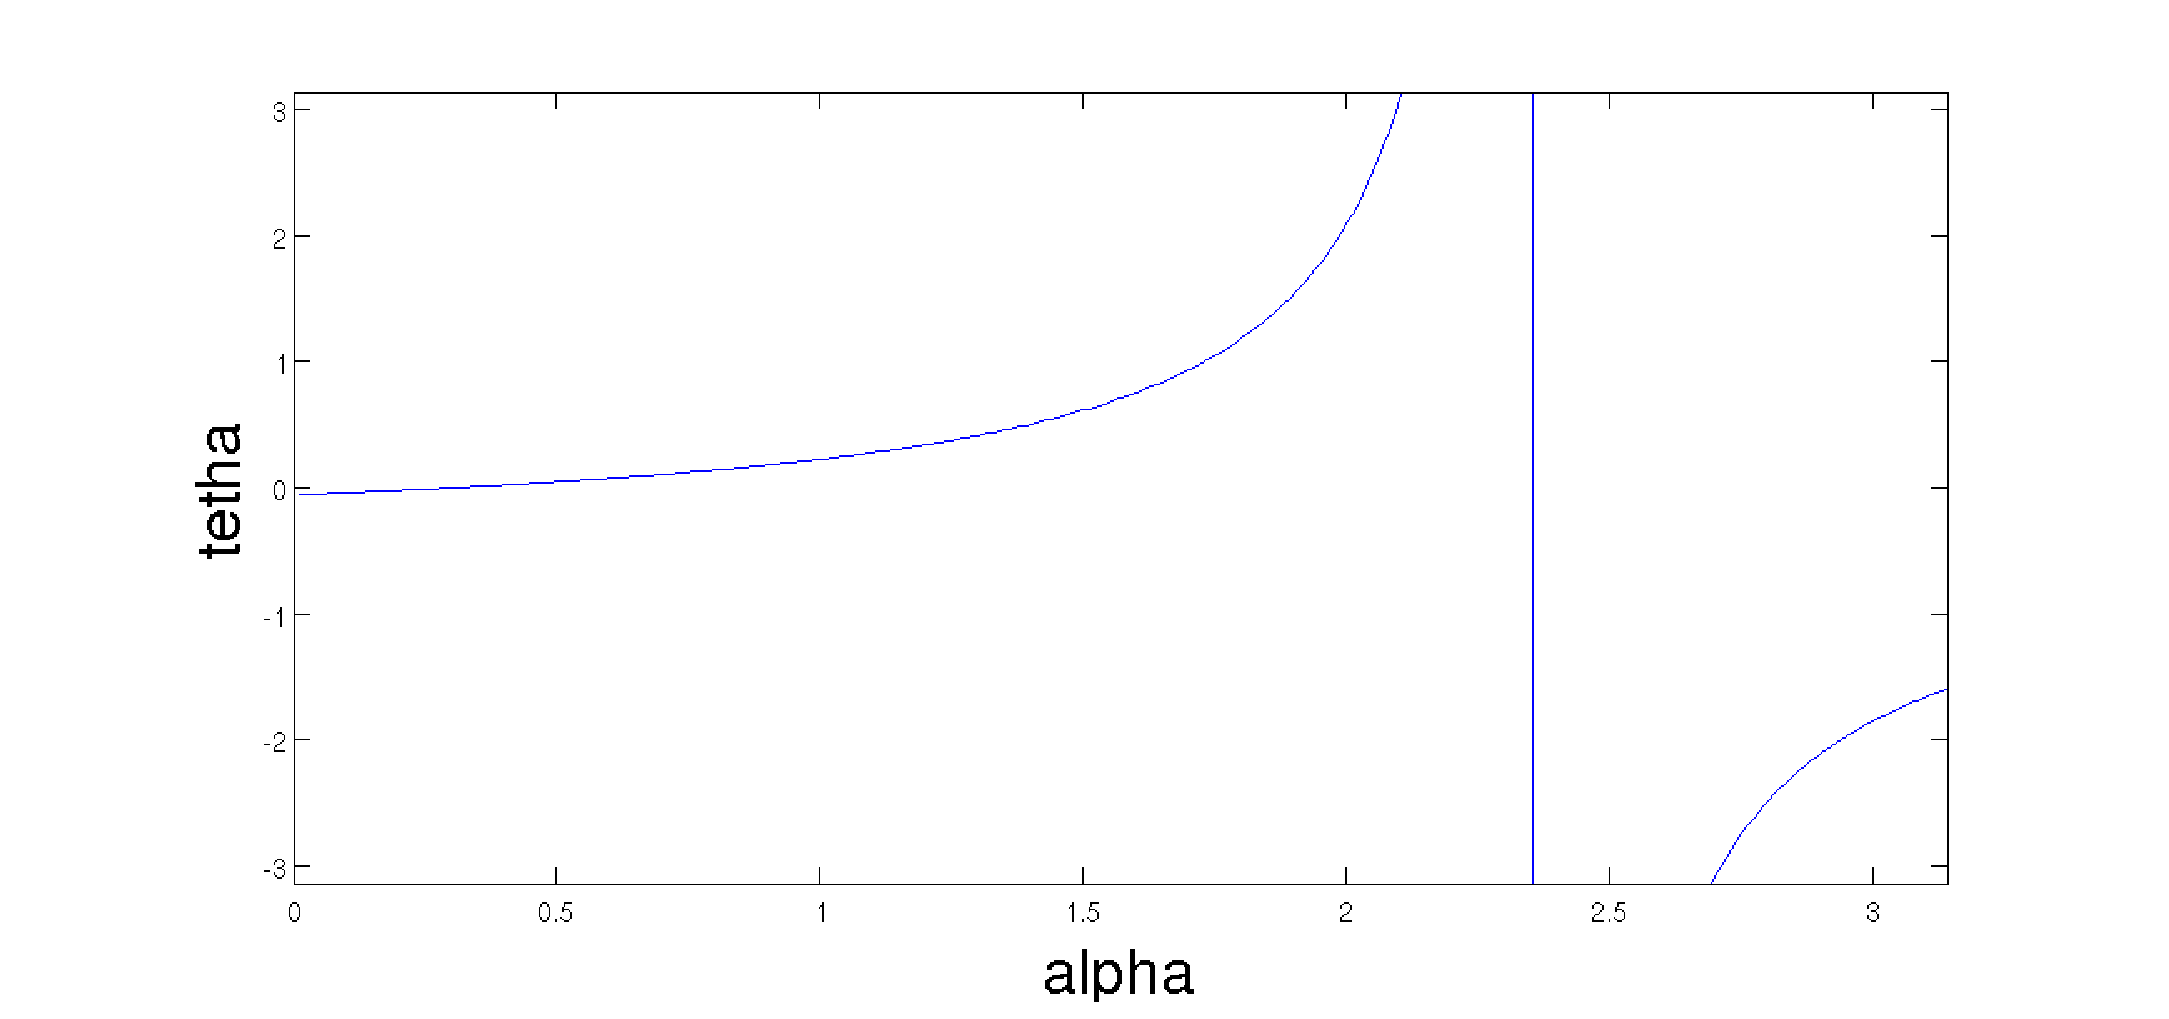
\includegraphics[width=1\columnwidth]{f_alpha}
  \caption{$\theta = f(\alpha)$.}
  \label{fig:f_alpha}
\end{figure}
 
